\section{Технический проект}
\subsection{Общая характеристика организации решения задачи}

Этот проект направлен на разработку системы, которая использует нечеткие нейронные сети для распознавания объектов на основе цветовых характеристик. Система будет способна анализировать изображения и выделять объекты, соответствующие заданным цветовым параметрам.

Основная цель - создание эффективной и точной системы распознавания объектов. Задачи включают:

\begin{itemize}
\item разработка алгоритма нечеткой нейронной сети;
\item создание базы данных для обучения и тестирования системы.
\end{itemize}

\subsection{Обоснование выбора технологии проектирования}

Нечеткие нейронные сети сочетают принципы нечеткой логики и нейронных сетей, что позволяет системе обрабатывать нечеткие и неточные данные, характерные для реальных изображений.

\subsubsection{Python и его библиотеки}

Python является предпочтительным языком программирования благодаря своей читаемости, простоте и обширной экосистеме библиотек, подходящих для работы с данными и машинным обучением:

\begin{enumerate}
\item NumPy. Используется для эффективной работы с массивами и матрицами, что критично для обработки изображений и численных вычислений.
\item Pandas. Предоставляет удобные структуры данных для анализа и манипуляции данными.
\item Matplotlib/Seaborn. Библиотеки для визуализации данных, которые помогают в анализе результатов и представлении данных.
\item OpenCV. Открытая библиотека для работы с компьютерным зрением, которая может использоваться для предварительной обработки изображений.
\item TensorFlow/Keras. Популярные фреймворки для глубокого обучения, которые предоставляют инструменты для создания, обучения и тестирования нейронных сетей.
\item Scikit-learn. Библиотека для машинного обучения, предоставляющая различные алгоритмы классификации, регрессии и кластеризации.
\end{enumerate}

\subsubsection{Архитектура нечёткой нейронной сети}

Архитектура нечеткой нейронной сети включает в себя 6 слоев с различными функциями.

Схема архитектуры нейронной сети представлена на рисунке ~\ref{neuro_diagram:image}.

\begin{figure}[ht]
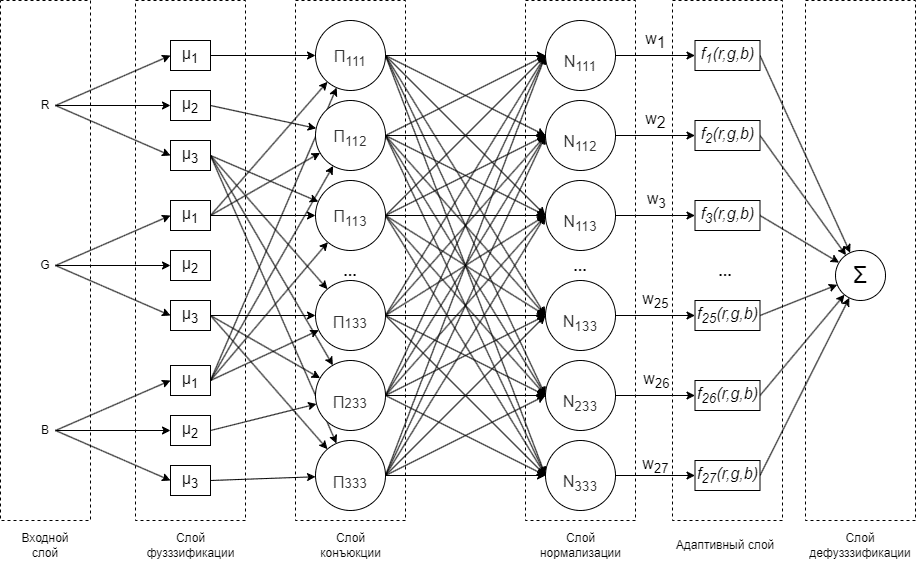
\includegraphics[width=1\linewidth]{neuro_diagram}
\caption{Схема архитектуры нейронной сети}
\label{neuro_diagram:image}
\end{figure}

Слои включают в себя:

\begin{enumerate}
\item Входной слой. В этом слое содержатся входные переменные, представленные 3 цветовыми каналами изображения. Эти переменные предоставляют исходную информацию для последующей обработки.

\item Слой фуpзификации. Он отвечает за преобразование значений яркости изображения в степени принадлежности. Здесь представлены функции принадлежности для каждой переменной, их количество равно 3 (яркие, средние или темные оттенки цвета), что в сумме создает 27 комбинаций. Функции принадлежности представлены гауссианами.

Вид функции Гаусса представлен на рисунке ~\ref{gaussmf:image}.

\begin{figure}[ht]
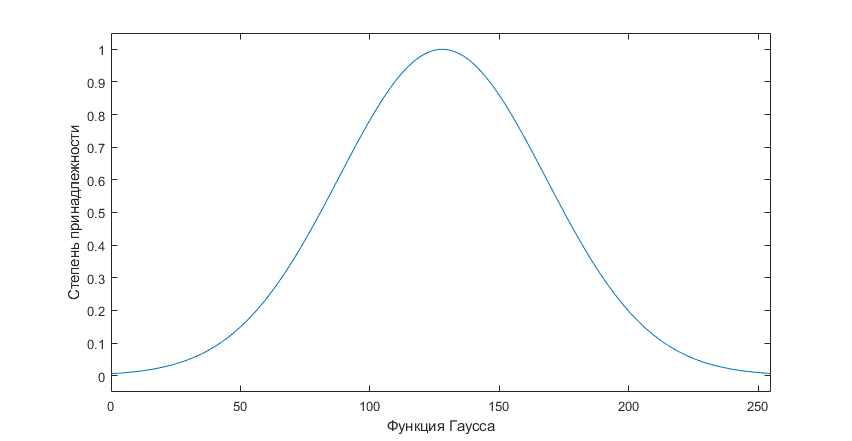
\includegraphics[width=1\linewidth]{gaussmf}
\caption{Функция Гаусса}
\label{gaussmf:image}
\end{figure}

\item Слой конъюнкции. На этом этапе происходит перемножение функций для каждой комбинации функций принадлежности по 3 цветовым каналам.

\item Слой нормализации. Здесь происходит нормализация полученных произведений.

\item Адаптивный слой. На этой стадии добавляются веса к нормализованным данным.

\item Слой дефузpификации. Здесь происходит суммирование всех функций для получения результата - яркости выходного пикселя.
\end{enumerate}

\subsubsection{Описание базы данных}

База данных будет хранить информацию о различных моделях обучения нейронной сети. У каждой модели будет своя таблица, в которой будут храниться данные об одном наборе обучения нейронной сети и одной таблице с уже обученными значениями. Каждый набор обучения будет содержать четыре столбца: три столбца для входных значений, соответствующих трем цветовым каналам изображения, и один столбец для выходных значений.

ERD диаграмма структуры базы данных представлена на рисунке ~\ref{databasediagram:image}.

\begin{figure}[ht]
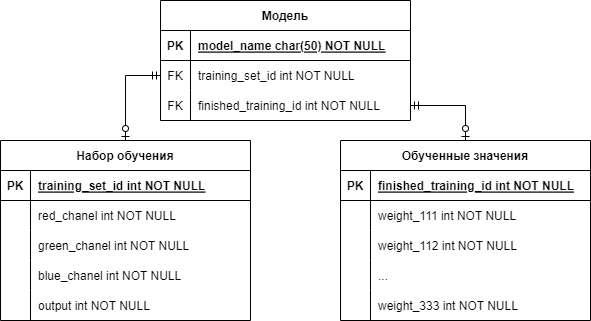
\includegraphics[width=1\linewidth]{databasediagram}
\caption{Диаграмма структуры базы данных}
\label{databasediagram:image}
\end{figure}

\subsection{Диаграмма компонентов}

Диаграмма компонентов представляет структуру системы в виде набора компонентов и их взаимосвязей. Каждый компонент отвечает за определенную функцию в рамках системы и может включать в себя подсистемы или модули.

\subsubsection{Структура компонентов}
На диаграмме компонентов изображены основные блоки системы, такие как:

\begin{enumerate}
\item Графический интерфейс пользователя. Модуль, отвечающий за взаимодействие с пользователем, представление результатов и получение входных данных.
\item Модуль предварительной обработки данных. Отвечает за подготовку данных к анализу, включая фильтрацию шума и нормализацию изображений.
\item Модуль нечеткой нейронной сети. Ядро системы, реализующее алгоритмы обучения и распознавания объектов.
\item База данных. Хранит обучающий и тестовый наборы данных, а также результаты работы системы.
\item Модуль анализа данных. Производит анализ данных, классификацию и предоставляет статистику по результатам.
\end{enumerate}

\subsubsection{Взаимодействие компонентов}
Компоненты системы взаимодействуют друг с другом следующим образом:

\begin{itemize}
\item пользователь загружает изображение через графический интерфейс пользователя;
\item интерфейс передает изображение в модуль предварительной обработки данных;
\item после обработки данные передаются в модуль нечеткой нейронной сети для распознавания объектов;
\item результаты распознавания сохраняются в базе данных;
\item модуль анализа данных извлекает результаты из базы данных и представляет их пользователю через графический интерфейс пользователя.
\end{itemize}

Диаграмма компонентов представленна на рисунке ~\ref{componentdiagram:image}.

\begin{figure}[ht]
\centering
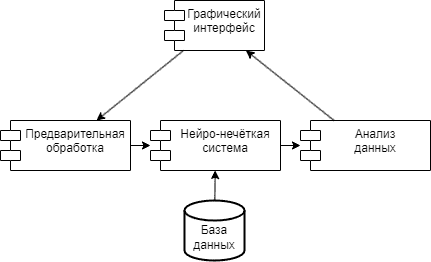
\includegraphics[width=0.7\linewidth]{componentdiagram}
\caption{Диаграмма компонентов системы}
\label{componentdiagram:image}
\end{figure}

\subsection{Содержание информационных блоков. Основные сущности}

Исходя из описания, можно выделить пять основных сущностей:

\begin{enumerate}
\item Графический интерфейс. Этот компонент отвечает за взаимодействие пользователя с нейронной сетью. Он представляет собой интерфейс, через который пользователь может отправлять данные на обработку, управлять обучающими данными нейронной сети и получать результаты.
\item Предварительная обработка. Эта сущность отвечает за предварительную обработку данных, поступающих от пользователя, чтобы подготовить их для дальнейшей работы нейронной сети. Здесь могут проводиться различные операции, такие как нормализация данных, фильтрация шума и преобразование формата.
\item Нейронная сеть. В данном участке происходит распознавание объектов на обработанном изображении с использованием выбранной модели или проведение обучения новой модели на выбранном наборе обучающих данных.
\item База данных. В этой части системы хранится информация о наборах обучающих данных и обученных моделях нейронной сети. База данных предоставляет доступ к данным для обучения и позволяет сохранять результаты работы нейронной сети для последующего использования.
\item Анализ данных. Этот компонент отвечает за анализ данных, полученных из нейронной сети. Здесь могут проводиться различные вычисления и визуализация результатов работы нейронной сети, а также их сохранение и представление пользователю.
\end{enumerate}

\subsubsection{Структура сущности графический интерфейс}
Графический интерфейс хранит в себе методы:

\begin{itemize}
\item запрос файла изображения у пользователя;
\item выбор нужного набра обучения, для обучения нейроной сети;
\item выбор нужной модели для расспознания объектов;
\item запуск обучения, который вызовет метод обучения из сущности нейронной сети;
\item запуск распознания, который вызовет метод обработки из сущности предварительной обработки;
\item запрос методов анализа данных, полученных из нейронной сети из сущности анализа данных.
\end{itemize}

\subsubsection{Структура сущности предварительная обработка}
Предварительная обработка осуществляет преобразование входящего изображения в формат, необходимый для работы нейронной сети.

\subsubsection{Структура сущности нейронная сеть}
Нейронная сеть строится в соответствии со структурой, описанной выше, и включает в себя два основных метода: обучение и распознавание объектов.

\subsubsection{Структура сущности база данных}
База данных предоставляет информацию для обучения и распознавания объектов нейронной сети, а также для сохранения новых обученных моделей.

\subsubsection{Структура сущности анализ данных}
Анализ данных включает в себя различные методы преобразования полученных от нейронной сети значений в полезные данные, такие как центры кластеров, количественное содержание цветов на изображении и другие.